Во время выполнения приложения могут возникать различные исключительные ситуации, которые могут пагубно сказаться на процессе работы приложения, поэтому эти ошибки необходимо предусмотреть и сделать их обработку.

Для возможности ввода данных в приложение используется обычные веб элементы ввода данных пример которого можно увидеть на рисунке~\ref{fig:input-empty}.

\begin{figure}[!h]
	\centering
	
\includegraphics[width=0.5\textwidth]{figures/input-empty.png}
	\caption{Стандартный блочный элемент ввода данных}
	\label{fig:input-empty}
\end{figure}

Разработанное приложение имеет встроенные валидаторы для того, чтобы пользователь не смог ввести данные, не предназначенные для конкретного поля. Например, если при обработке численных значений (присваивании значений в поля численных данных, выполнении математических операций) в незащищённое приложение ввести текст, то при попытке преобразований пользователь получит сообщение о критической ошибке, как показано на рисунке~\ref{fig:input-invalid}.

\begin{figure}[!h]
	\centering
	
\includegraphics[width=0.5\textwidth]{figures/input-invalid.png}
	\caption{Уведомление об неверно введенных данных}
	\label{fig:input-invalid}
\end{figure}

Благодаря инструмента валидации включенным в фреймворк \textit{Angular~7} можно легко валидировать \textit{HTML} элементы в форме отправки запросов, что максимально исключает вероятность экстренного прекращения работы разработанного приложения. На рисунке~\ref{fig:validation-code} показан код на языке \textit{TypeScript}, который выполняет проверку полей формы.

\begin{figure}[!h]
	\centering
	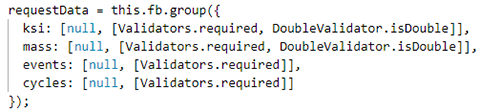
\includegraphics[width=\textwidth]{figures/validation-code.png}
	\caption{Код валидации формы}
	\label{fig:validation-code}
\end{figure}

Моделирование столкновений протонов занимает много процессорного времени и для того, чтобы снизить загруженность вычислительной системы имитационным моделированием было решено сделать верификацию и кэширование уже рассчитанных результатов. 

Данные в кэше хранятся на устройстве с быстрым доступом и могут использоваться совместно с программными компонентами. Основная функция кэша – ускорение процесса извлечения данных. Он избавляет от необходимости проводить имитационное моделирование вновь и вновь для одинаковых начальных условий.

Данная задача легко решается по средствам стандартных инструментов кэширования фреймворка \textit{Spring}, как показано на рисунке~\ref{fig:cache} необходимо лишь подключить аннотацию фреймворка.

\begin{figure}[!h]
	\centering
	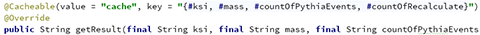
\includegraphics[width=\textwidth]{figures/cache.png}
	\caption{Код кэширования результата имитационного моделирования}
	\label{fig:cache}
\end{figure}

Сохрание результата метода \textit{getResult} для сервиса \textit{ZprimeServiceImpl} достаточно, чтобы все результаты вычислений были сохранены. Так же необходимо указать базу данных для хранения кэш данных. В разработанном приложении была использована база данных \textit{Redis}.

\textit{Redis} (\textit{REmote DIctionary Server}) -- это нереляционная высокопроизводительная СУБД. \textit{Redis} хранит все данные в памяти, доступ к данным осуществляется по ключу. Опционально копия данных может храниться на диске. Этот подход обеспечивает производительность, в десятки раз превосходящую производительность реляционных СУБД, а также упрощает секционирование (шардинг) данных.

Важным моментом в реализации архитектуры разработанного приложения является возможность экспорта сохраненных данных из приложения (\textit{persistence}). \textit{Persistence Data} -- это данные, сохраняющиеся в информационной системе в течение более одного сеанса управления данными. Компания \textit{Amazon} предлагает широкий набор различных готовых решений в том числе и решение для сохранения данных между сеансами разработанного приложения называемое \textit{AWS ElastiCache}. Данный сервис позволяет легко экпортировать данные из базы \textit{Redis} в \textit{Amazon S3 backet}, как показано на рисунке~\ref{fig:elasti-cache}. 

\begin{figure}[!h]
	\centering
	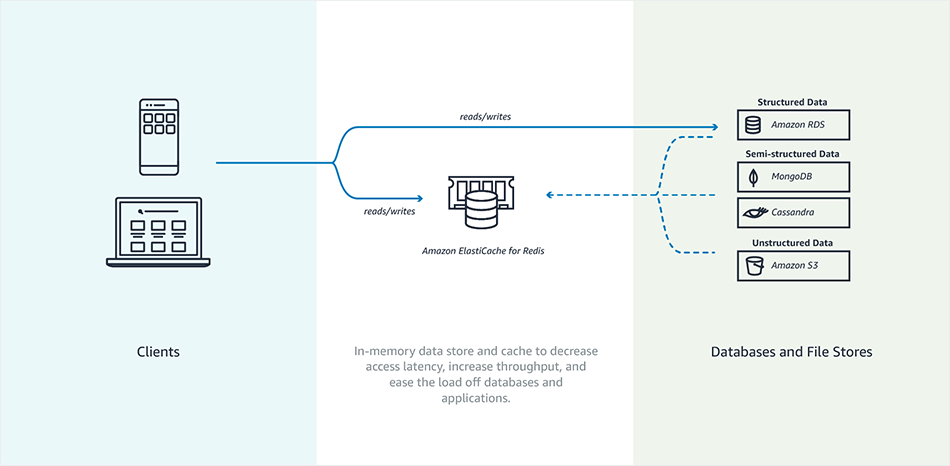
\includegraphics[width=\textwidth]{figures/elasti-cache.png}
	\caption{Работа с данными в \textit{AWS ElastiCache}}
	\label{fig:elasti-cache}
\end{figure}

\textit{Amazon S3} (\textit{Amazon Simple Storage Service}) позволяет хранить контент и получать к нему доступ из любого места в любое время. \textit{Amazon S3} хранит данные в виде объектов в корзинах (\textit{bucket}). Каждый объект представляет собой файл и, опционально — метаданные, которые этот объект описывают. Корзина — это контейнер, который хранит объекты. Можно иметь неограниченное количество таких корзин, и для каждой — установить доступ (кто может создавать, удалять и просматривать список объектов в корзине), просматривать логи доступа к корзине и объектам в ней.



% обратчик исключительных ситуаций в спринге